%%%
\subsection{Feature Engineering}

From the features in the dataset, we can create new features that may be relevant, like ``Rush Hour,'' combining hour with day of week.  During rush hour, the number of crashes increases, but their average severity goes down.  We drew the lines distinguishing ``Rush Hour'' from "Not Rush Hour'' based, again, on the correlation to hospitalization.  Interestingly, the hospitalization rates varied by age, and varied by sex, but varied differently by age within sex.  Hospitalization rates for young children are low, perhaps due to child seat requirements, but after young childhood, as age increases, the hospitalization rate increases for both men and women, but younger women have a lower hospitalization rate than men, and older women have a higher rate.  We created an \verb|AGE_SEX| feature.  


\begin{center}

\begin{tabular}{lrrr}
\multicolumn{4}{c}{Crash Person Count} \cr
\toprule
{Age} &  Female &    Male &   Total \\
\midrule
00-06 &   12331 &   12639 &   24970 \\
07-15 &   16623 &   16726 &   33349 \\
16-18 &   20158 &   21622 &   41780 \\
19-52 &  175528 &  219931 &  395459 \\
53-70 &   49750 &   65228 &  114978 \\
71+   &   15972 &   17766 &   33738 \\ \hline
Total &  290362 &  353912 &  644274\vrule width 0pt height 10pt \\
\bottomrule
\end{tabular}
\end{center}

\begin{center}
\begin{tabular}{lrrr}
\multicolumn{4}{c}{Hospitalization Count} \cr
\toprule
{Age} &  Female &   Male &   Total \\
\midrule
00-06 &    1448 &   1560 &    3008 \\
07-15 &    2529 &   2779 &    5308 \\
16-18 &    2900 &   2998 &    5898 \\
19-52 &   28843 &  33514 &   62357 \\
53-70 &    9302 &  10947 &   20249 \\
71+   &    3503 &   3287 &    6790 \\ \hline
Total &   48525 &  55085 &  103610\vrule width 0pt height 10pt \\
\bottomrule
\end{tabular}
\end{center}

\begin{center}
\begin{tabular}{lrrr}
\multicolumn{4}{c}{Hospitalization Rate} \cr
\toprule
{Age} &  Female &   Male &  Total \\
\midrule
00-06 &   0.117 &  0.123 &  0.240 \\
07-15 &   0.152 &  0.166 &  0.318 \\
16-18 &   0.144 &  0.139 &  0.283 \\
19-52 &   0.164 &  0.152 &  0.316 \\
53-70 &   0.187 &  0.168 &  0.355 \\
71+   &   0.219 &  0.185 &  0.404 \\ \hline
Total &   0.983 &  0.933 &  1.916\vrule width 0pt height 10pt \\
\bottomrule
\end{tabular}
\end{center}

\begin{center}
\begin{tabular}{lrrr}
\multicolumn{4}{c}{Rate Normalized by Row} \cr
\toprule
{Age} &  Female &   Male &  Total \\
\midrule
00-06 &   0.488 &  0.512 &    1.0 \\
07-15 &   0.478 &  0.522 &    1.0 \\
16-18 &   0.509 &  0.491 &    1.0 \\
19-52 &   0.519 &  0.481 &    1.0 \\
53-70 &   0.527 &  0.473 &    1.0 \\
71+   &   0.542 &  0.458 &    1.0 \\ \hline
Total &   3.063 &  2.937 &    6.0\vrule width 0pt height 10pt \\
\bottomrule
\end{tabular}
\end{center}

\begin{center}
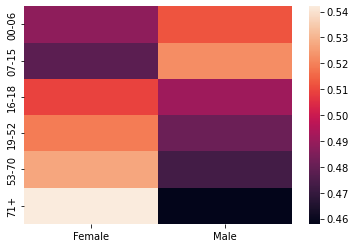
\includegraphics[scale=0.6]{AGE_IM_SEX_IM_Row.png}

Hospitalization Rate Normalized by Age
\end{center}

For full details see the code \verb|CRSS_05_24_22_Crosstabs|.
